%%%%%%%%%%%%%%%%%%%%%%%%%%%%%%%%%%%%%%%%%%

\appendixtitles{no}
\appendixstart
\appendix
\section[\appendixname]{}

\begin{figure*}

{\centering 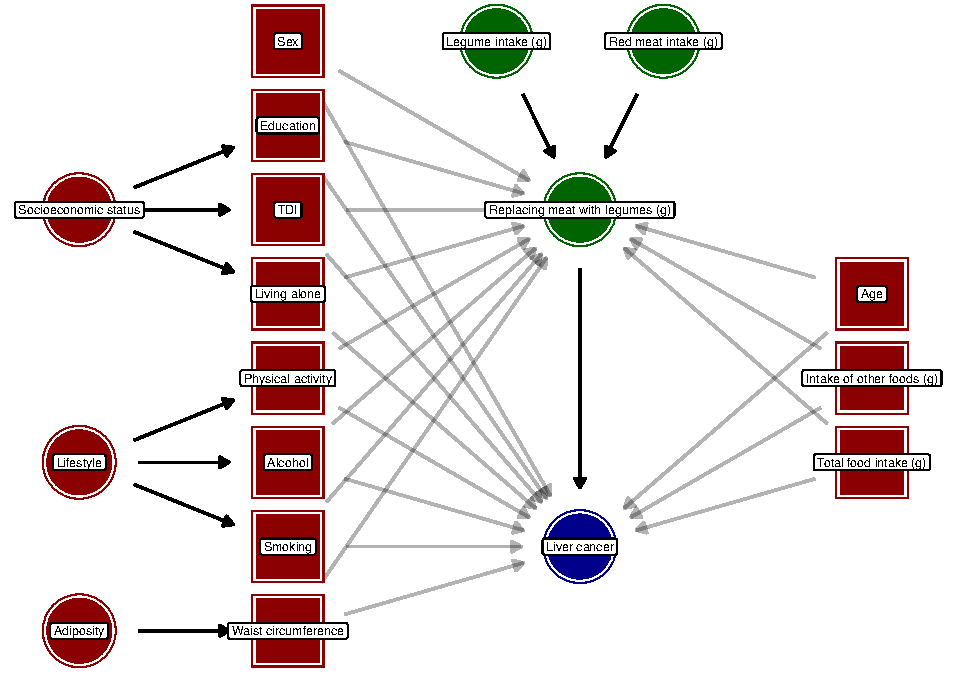
\includegraphics[width=1\linewidth,]{appendix-test_files/figure-latex/fig2-1}

}

\caption{Simplified directed acyclic graph (DAG) visualizing the hypothesised causal relationship between replacing red meat with legumes and liver cancer based on assumptions of biasing paths. Red nodes represent confounders. Square nodes represent the minimal sufficient adjustment set for estimating the effect of replacing red meat with legumes on liver cancer. Shadowed arrows represent biasing paths. DAG terminology demands visualisation of all hypothesized correlating relationships between variables, typically resulting in complex and hard-to-follow illustrations. To improve readability, inter-covariate arrows are hidden in the above DAG.}\label{fig:fig2}
\end{figure*}

\begin{table}[t]
\caption{
\label{tab:food-group}\textbf{Supplementary table 1. Summary of included foods for each food group.}}
\fontsize{9.0pt}{10.8pt}\selectfont
\begin{tabular*}{1\linewidth}{@{\extracolsep{\fill}}>{\raggedright\arraybackslash}p{\dimexpr 0.2\linewidth-2\tabcolsep-1.5\arrayrulewidth}>{\raggedright\arraybackslash}p{\dimexpr 0.8\linewidth-2\tabcolsep-1.5\arrayrulewidth}}
\toprule
\textbf{Food group} & \textbf{Includes} \\
\midrule\addlinespace[2.5pt]
{\bfseries Legumes} & Soya-based desserts, Baked beans, pulses, Soya drinks (including calcium fortified),
  Tofu-based products, Hummus, Peas \\
{\bfseries Red meat} & Beef, Lamb, Other meat including offal, Pork \\
{\bfseries Processed meat} & Sausages, bacon (with and without fat), ham, liver pate \\
{\bfseries Animal-based foods} & Poultry, fish, dairy, eggs, mixed dishes, and sauces and condiments \\
{\bfseries Healthy plant-based foods} & Whole grains, fruits, nuts, plant oils, beverages (water, tea and coffee), vegetables \\
{\bfseries Unhealthy plant-based foods} & Refined cereals, potatoes, fruit juice, mixed dishes (vegetarian), sweets \& snacks, and sugar sweetened beverages \\
{\bfseries Alcoholic beverages} & Beer and cider, spirits and other alcoholic drinks, fortified wine, red and rose wine, white wine \\
\bottomrule
\end{tabular*}
\end{table}

\begin{table}[t]
\caption{
\label{tab:cancer}\textbf{Replacing 15/day of total meat, red meat and processed meat with legumes and hazard ratios and 95\% confidence intervals for hepatocellular carcinoma and intrahepatic cholangiocarcinoma.}}
\fontsize{9.0pt}{10.8pt}\selectfont
\begin{tabular*}{1\linewidth}{@{\extracolsep{\fill}}lcc}
\toprule
 & \textbf{Model 1}\textsuperscript{\textit{1}} & \textbf{Model 2}\textsuperscript{\textit{2}} \\
\cmidrule(lr){2-2} \cmidrule(lr){3-3}
\textbf{15 g/day of legumes replacing:} & \textbf{HR} \textbf{(95\% CI)} & \textbf{HR} \textbf{(95\% CI)} \\
\midrule\addlinespace[2.5pt]
\multicolumn{3}{l}{{\bfseries Hepatocellular carcinoma}} \\
\midrule\addlinespace[2.5pt]
Total red meat & 1.02 (0.94-1.11) & 1.06 (0.97-1.16) \\
Unprocessed red meat & 1.02 (0.93-1.11) & 1.04 (0.95-1.15) \\
Processed red meat & 1.04 (0.90-1.19) & 1.10 (0.96-1.27) \\
\midrule\addlinespace[2.5pt]
\multicolumn{3}{l}{{\bfseries Intrahepatic cholangiocarcinoma}} \\
\midrule\addlinespace[2.5pt]
Total red meat & 0.94 (0.87-1.02) & 0.97 (0.89-1.05) \\
Unprocessed red meat & 0.92 (0.85-1.00) & 0.94 (0.87-1.02) \\
Processed red meat & 1.03 (0.90-1.18) & 1.07 (0.93-1.23) \\
\bottomrule
\end{tabular*}
\begin{minipage}{\linewidth}
\textsuperscript{\textit{1}}Multivariate Cox proportional hazards regression model adjusted for age (as underlying timescale), other food groups, and total food intake.\\
\textsuperscript{\textit{2}}Further adjusted for sex, educational level, Townsend deprivation index, living alone, physical activity, smoking, alcohol intake, and waist circumference.\\
\end{minipage}
\end{table}

\begin{table}[t]
\caption{
\label{tab:legume}\textbf{No intake of legumes vs. quartiles of daily legume intake and hazard ratios and 95\% confidence intervals for primary liver cancer.}}
\fontsize{9.0pt}{10.8pt}\selectfont
\begin{tabular*}{1\linewidth}{@{\extracolsep{\fill}}lccc}
\toprule
 &  & \textbf{Model 1}\textsuperscript{\textit{1}} & \textbf{Model 2}\textsuperscript{\textit{2}} \\
\cmidrule(lr){3-3} \cmidrule(lr){4-4}
\textbf{Characteristic} & \textbf{Mean daily legume intake} & \textbf{HR} \textbf{(95\% CI)} & \textbf{HR} \textbf{(95\% CI)} \\
\midrule\addlinespace[2.5pt]
Categories: &  &  &  \\
    No intake & 0.00 & — & — \\
    Q1 & 6.3 & 0.59 (0.35-0.98) & 0.60 (0.36-0.99) \\
    Q2 & 16 & 0.88 (0.57-1.35) & 0.90 (0.58-1.38) \\
    Q3 & 34 & 0.73 (0.46-1.17) & 0.74 (0.47-1.19) \\
    Q4 & 109 & 0.98 (0.64-1.52) & 1.07 (0.69-1.66) \\
\bottomrule
\end{tabular*}
\begin{minipage}{\linewidth}
\textsuperscript{\textit{1}}Multivariate Cox proportional hazards regression model adjusted for age (as underlying timescale), other food groups, and total food intake.\\
\textsuperscript{\textit{2}}Further adjusted for sex, educational level, Townsend deprivation index, living alone, physical activity, smoking, alcohol intake, and waist circumference.\\
\end{minipage}
\end{table}

\clearpage
\startlandscape

\begin{table}[t]
\caption{
\label{tab:sens}\textbf{Sensitivity analyses}}
\fontsize{7.5pt}{9.0pt}\selectfont
\begin{tabular*}{1\linewidth}{@{\extracolsep{\fill}}>{\raggedright\arraybackslash}p{\dimexpr 0.125\linewidth-2\tabcolsep-1.5\arrayrulewidth}>{\centering\arraybackslash}p{\dimexpr 0.125\linewidth-2\tabcolsep-1.5\arrayrulewidth}>{\centering\arraybackslash}p{\dimexpr 0.125\linewidth-2\tabcolsep-1.5\arrayrulewidth}>{\centering\arraybackslash}p{\dimexpr 0.125\linewidth-2\tabcolsep-1.5\arrayrulewidth}>{\centering\arraybackslash}p{\dimexpr 0.125\linewidth-2\tabcolsep-1.5\arrayrulewidth}>{\centering\arraybackslash}p{\dimexpr 0.125\linewidth-2\tabcolsep-1.5\arrayrulewidth}>{\centering\arraybackslash}p{\dimexpr 0.125\linewidth-2\tabcolsep-1.5\arrayrulewidth}>{\centering\arraybackslash}p{\dimexpr 0.125\linewidth-2\tabcolsep-1.5\arrayrulewidth}}
\toprule
 & \multicolumn{5}{c}{\textbf{Exclusion of participants with:}} &  &  \\
\cmidrule(lr){2-6}
 & \textbf{High alcohol intake}\textsuperscript{\textit{1}} & \textbf{Implausible food intake}\textsuperscript{\textit{2}} & \textbf{Liver disease before baseline}\textsuperscript{\textit{3}} & \textbf{Any cancer before baseline}\textsuperscript{\textit{4}} & \textbf{Fewer than 3 Oxford WebQs} & \textbf{Death register as source of liver cancer events} & \textbf{Exclusion of waist circumference from analysis} \\
\cmidrule(lr){2-2} \cmidrule(lr){3-3} \cmidrule(lr){4-4} \cmidrule(lr){5-5} \cmidrule(lr){6-6} \cmidrule(lr){7-7} \cmidrule(lr){8-8}
\textbf{15 g/day of legumes replacing:} & \textbf{HR} \textbf{(95\% CI)} & \textbf{HR} \textbf{(95\% CI)} & \textbf{HR} \textbf{(95\% CI)} & \textbf{HR} \textbf{(95\% CI)} & \textbf{HR} \textbf{(95\% CI)} & \textbf{HR} \textbf{(95\% CI)} & \textbf{HR} \textbf{(95\% CI)} \\
\midrule\addlinespace[2.5pt]
Total red meat & 1.00 (0.94-1.06) & 1.01 (0.95-1.07) & 0.99 (0.93-1.06) & 1.03 (0.96-1.11) & 1.04 (0.96-1.12) & 1.02 (0.96-1.08) & 1.00 (0.94-1.06) \\
Unprocessed red meat & 0.98 (0.92-1.05) & 0.99 (0.93-1.05) & 0.97 (0.90-1.04) & 1.00 (0.93-1.08) & 1.02 (0.94-1.11) & 1.00 (0.94-1.07) & 0.98 (0.92-1.05) \\
Processed red meat & 1.06 (0.95-1.18) & 1.08 (0.98-1.20) & 1.08 (0.96-1.20) & 1.15 (1.01-1.30) & 1.11 (0.97-1.27) & 1.07 (0.98-1.18) & 1.06 (0.96-1.17) \\
\bottomrule
\end{tabular*}
\begin{minipage}{\linewidth}
\textsuperscript{\textit{1}}Exclusion of the upper decile of alcohol intake (g/day) by sex.\\
\textsuperscript{\textit{2}}Exclusion of participants below the 2.5th percentile and above the 97.5th percentile of energy intake (kJ/day) by sex.\\
\textsuperscript{\textit{3}}ICD10 codes: K70-79, B16-19, Z94.4, I85, I86.4, and E83.0-1. ICD9 codes: 5710-5745, 0700-0709, V427 and 2750-2751.\\
\textsuperscript{\textit{4}}ICD10 codes: C00-C97 and D00-D48. ICD9 codes: 140-239.\\
\end{minipage}
\end{table}

\finishlandscape
